\documentclass[12pt,a4paper]{article}

% ── Packages ──────────────────────────────────────────────────────────────────
\usepackage[margin=2.5cm]{geometry}
\usepackage{graphicx}
\usepackage{amsmath}
\usepackage{booktabs}
\PassOptionsToPackage{hyphens}{url}
\usepackage{hyperref}
\usepackage{xurl}
\usepackage{xcolor}
\usepackage{listings}
\usepackage{enumitem}
\usepackage{caption}
\usepackage{subcaption}
\usepackage{tikz}
\usepackage{pgfplots}
\pgfplotsset{compat=1.18}
\usetikzlibrary{shapes.geometric, arrows.meta, positioning, fit, backgrounds, calc}
\usepackage[numbers,sort&compress]{natbib}
\usepackage{microtype}
\usepackage{lineno}
\usepackage{setspace}
\doublespacing

\definecolor{argblue}{RGB}{26,79,138}
\definecolor{apsorange}{RGB}{232,119,34}
\definecolor{codegray}{RGB}{245,245,245}

\lstset{
  basicstyle=\ttfamily\small,
  backgroundcolor=\color{codegray},
  frame=single,
  framesep=4pt,
  breaklines=true,
  columns=fullflexible,
}

\hypersetup{
  colorlinks=true,
  linkcolor=argblue,
  citecolor=argblue,
  urlcolor=argblue,
  breaklinks=true,
}

% ── Title block ────────────────────────────────────────────────────────────────
\title{\textbf{Query-GSAS: A Local Retrieval-Augmented Generation System
       for Intelligent Access to GSAS-II Documentation}}

\author{
  Pawan K. Tripathi$^{\ast}$ \and
  Mathew J.\ Cherukara \and
  Brian H.\ Toby$^{\ast}$
}

\date{
  X-ray Science Division, Advanced Photon Source,
  Argonne National Laboratory, Lemont, IL 60439, USA \\[4pt]
  $^{\ast}$Correspondence: \href{mailto:ptripathi@anl.gov,toby@anl.gov}{ptripathi@anl.gov, toby@anl.gov}
}

% ── Document ───────────────────────────────────────────────────────────────────
\begin{document}

\maketitle
\linenumbers

\begin{abstract}
  GSAS-II, a widely-used package for powder and single-crystal
diffraction analysis, is supported by an extensive set of tutorials, help pages,
and reference documents totalling $\sim$500,000 words across five source categories comprising 331 HTML files.
Navigating this wealth of documentation presents challenges for new and experienced users alike.
We present \textit{Query-GSAS}, a retrieval-augmented generation (RAG)
system that provides natural-language access to the complete GSAS-II
documentation corpus.
Source documents are ingested into a local vector database; at query time, semantically relevant passages are retrieved by dense embedding search and a large language model (LLM) synthesises a fluent, cited answer from those passages.
Four backends are supported: an Ollama server (using any model available via
\texttt{ollama pull}), \texttt{llama-cpp-python} for in-process GGUF
inference requiring no separate server process, an Anthropic API option, and a retrieval-only mode that returns raw documentation passages without LLM synthesis.
A post-processing citation injector connects every substantive claim in
the generated response to the original GSAS-II source document by inserting
an inline marker providing a reference to a ranked bibliography below the response.
In the web UI, these are clickable hyperlinks.
\textit{Query-GSAS} is incorporated into GSAS-II using a separate wxPython dialog window, but can also be run as a separate utility offering alternative user interfaces, including a command-line tool and a browser-based interface that uses a self-contained FastAPI web application. \textit{Query-GSAS} can be run as a fully local architecture, which satisfies the security and data-residency requirements of research facilities that require air-gapped or high-performance computing environments. The package serves as a model for how to develop natural-language documentation search tools for other large scientific packages. 
\end{abstract}

\noindent\textbf{Keywords:} retrieval-augmented generation; GSAS-II;
powder diffraction; Rietveld refinement; large language models;
crystallographic software; documentation

\clearpage

\input{sections/introduction}
\section{System Design and Implementation}
\label{sec:methods}

Figure~\ref{fig:architecture} shows the overall system architecture.
\textit{Query-GSAS} is structured around four loosely coupled components:
a documentation ingestion pipeline, a persistent vector store,
a retrieval and ranking engine, and a generation backend.
All components can be run on the user's local machine. Thus, it can be run in a manner where no data leaves the host at any point, even on an air-gapped computer.

% ── 2.1 Documentation corpus ─────────────────────────────────────────────────
\subsection{Documentation corpus and ingestion}
\label{sec:corpus}

\subsubsection{Source catalogue}

The GSAS-II documentation is distributed across several publicly accessible
web servers.
Table~\ref{tab:sources} summarises the sources included in the index.

\begin{table}[h]
  \centering
  \caption{Documentation HTML files indexed by \textit{Query-GSAS}.}
  \label{tab:sources}
  \begin{tabular}{lccc}
    \toprule
    Category & Files & Words & Chunks \\
    \midrule
    Home pages (installation, etc.)    & 22 & 22K & 329 \\
    Help manual sections               & 42 & 54K & 554 \\
    Tutorials (dynamically fetched)    & 65 & 167K & 1{,}437 \\
    Programmer's Guide (ReadTheDocs)   & 23 & 143K & 2{,}740 \\
    Powder Crystallography textbook    & 179 & 115K  & 778 \\
    \midrule
    \textit{Total}                     & 331 & 501K & 5{,}838 \\
    \bottomrule
  \end{tabular}
\end{table}

Tutorial URLs are resolved dynamically at ingest time by fetching from the project
repository the
GSAS-II canonical \texttt{tutorialIndex.py} file that is used within GSAS-II for 
indexing the tutorials. The URL list is extracted via \texttt{ast.literal\_eval}
--- avoiding \texttt{eval}/\texttt{exec} for security.
This ensures that newly published tutorials are automatically included
without manual source-list maintenance. 
While two larger documents are available as monolithic PDF files, and \textit{Query-GSAS} is able to ingest the content in that format, we have found that paginated HTML content is preferable for this purpose, as \textit{Query-GSAS} is then able to guide users to the appropriate documentation section and then open that resource for them in a browser. Further, use of HTML preserves hyperlinks, section
headings, and code-block formatting that are degraded by PDF parsing.
In HTML form, the Programmer's Guide is provided as 23 individual HTML pages on the ReadTheDocs service
\url{https://gsas-ii.readthedocs.io/en/latest/}, one per module. Both the PDF and HTML forms are generated whenever the GSAS-II source code is updated on GitHub.
The \textit{Powder Diffraction Crystallography} textbook\citep{toby2024book}, under development, has been formatted as a series of HTML pages specifically for use in \textit{Query-GSAS} and the pages are hosted via the book repository's GitHub Pages site.
The HTML will be rebuilt from the \LaTeX\ sources each time a new book edition is tagged.
The naming pattern used for the generated web pages of the Powder Crystallography textbook allows the indexing routine to find the full contents without hard-coding all the file names. 

\subsubsection{Ingestion pipeline}

Each HTML source is fetched with the \texttt{requests} library and
parsed using \texttt{BeautifulSoup4} with the \texttt{lxml} backend.
Boilerplate elements (navigation bars, footers, scripts, and images)
are removed, and the remaining content is segmented into sections by
heading level (H1--H4).
PDF documents, when included, are parsed using the \texttt{pypdf} module, with pages
batched in groups of three to maintain cross-page contextual continuity.

Sections are divided into overlapping text chunks using a
sentence-boundary aware splitting algorithm: each chunk is at most
1{,}200 characters with a 150-character overlap, and splits are
placed at the nearest preceding sentence boundary within the
sliding window, avoiding severed mid-sentence context.
Each chunk is assigned a content-hash identifier derived from the
MD5 digest of its source URL, section heading, and full text content,
enabling idempotent \texttt{upsert} operations: re-running ingestion
on an already-indexed source updates only modified chunks.

Embeddings are produced using the \texttt{BAAI/bge-base-en-v1.5}
model \citep{bge2023embedding} served via the \texttt{fastembed} ONNX
runtime, which requires no PyTorch installation.
This model produces 768-dimensional dense vectors and consistently
outperforms the smaller \texttt{all-MiniLM-L6-v2}
\citep{wang2020minilm,reimers2019sbert} on domain-specific retrieval
benchmarks while remaining practical for CPU-only deployment.
Full ingestion of all HTML sources in Table \ref{tab:sources} completes in approximately
30 minutes on a modern laptop CPU and produces a $\sim$65\,MB database. To avoid the demands for running this indexing process, a GitHub Action is used to generate this weekly and a zip-compressed copy of the database made available. When \textit{Query-GSAS} is run from inside GSAS-II, the user is offered the option to download the database. 

% ── 2.2 Vector store ─────────────────────────────────────────────────────────
\subsection{Vector store}

Embeddings, raw text, and per-chunk metadata (source URL, page title,
section heading, and source category) are stored in a ChromaDB
\citep{chromadb2023} persistent collection using the cosine similarity
metric.
The index is stored locally at \texttt{\textasciitilde/.GSASII/query\_gsas2/chroma\_db}
by default, co-located with other GSAS-II user data and separating it
from the package installation.
The storage location can be overridden via the
\texttt{GSAS\_QUERY\_DATA\_DIR} environment variable.

ChromaDB is selected over alternatives (FAISS, Qdrant, Milvus) because
it requires no external service process, stores data as a portable
SQLite database alongside raw vector files, and supports incremental
\texttt{upsert} operations that make re-indexing individual updated
sources efficient.

% ── 2.3 Retrieval ────────────────────────────────────────────────────────────
\subsection{Retrieval and ranking}
\label{sec:retrieval}

At query time, the user's question is embedded using the same
\texttt{BAAI/bge-base-en-v1.5} model (loaded once and cached in memory via
\texttt{functools.lru\_cache}) and the top 30 nearest vectors are
initially retrieved by approximate nearest-neighbour search.
To maximise source diversity, a URL-deduplication step retains only
the highest-scoring chunk from each unique source page; the resulting
ranked list is then truncated to the top six chunks forwarded to the
generation backend.
Retrieved scores are linearly normalised within the selected set:
the best-matching chunk is assigned relevance 1.0 and the weakest 0.0,
with intermediate chunks scaled proportionally.
These normalised scores are provided to the user in the answer UI.


% ── 2.4 Generation ───────────────────────────────────────────────────────────
\subsection{Text generation and source citation}
\label{sec:inference}

\textit{Query-GSAS} supports four text generation backends selected via the
\texttt{LLM\_BACKEND} environment variable (Table~\ref{tab:backends}).
Priority order when \texttt{LLM\_BACKEND} is unset: if
\texttt{llama-cpp-python} is importable it is selected automatically;
otherwise Ollama is used.

\begin{table}[h]
  \centering
  \caption{Supported generation backends.}
  \label{tab:backends}
  \begin{tabular}{llll}
    \toprule
    Backend & Default model & Data locality & Notes \\
    \midrule
    \texttt{ollama}      & Llama 3 8B            & Fully local & Separate server process \\
    \texttt{llama\_cpp}  & Any GGUF model        & Fully local & In-process; no daemon \\
    \texttt{anthropic}   & Claude Sonnet 4       & External API & API key required \\
    \texttt{retrieval}   & ---                   & Fully local & No LLM; raw chunks \\
    \bottomrule
  \end{tabular}
\end{table}

The \textbf{Ollama} backend \citep{ollama2023} serves quantised large
language models on consumer hardware via a local REST API.
Any model available via \texttt{ollama pull} can be substituted
(\emph{e.g.}\ Mistral 7B, Qwen2.5 7B, Llama 3 70B) by setting environment variable 
\texttt{OLLAMA\_MODEL}.
The default for this, the Llama 3 8B model, \citep{meta2024llama3}, in 4-bit quantisation
requires approximately 5\,GB of storage and 6\,GB of RAM.
The wxPython GUI initiates and ends the Ollama server process
automatically with the dialog window lifecycle, registering a
\texttt{atexit} handler to ensure clean termination even when
GSAS-II exits without closing the assistant dialog.

The \textbf{\texttt{llama-cpp-python}} backend \citep{llamacpp2023}
loads GGUF model files in-process, requiring no separate server daemon.
It is auto-detected at startup and selected over Ollama when
\texttt{llama-cpp-python} can be imported and \texttt{LLM\_BACKEND}
is not set.
The model is loaded once and cached via
\texttt{@lru\_cache(maxsize=1)}, avoiding the 3--5\,s
reload penalty on each query.
Tested with Qwen2.5-3B-Instruct \citep{qwen2025} Q4\_K\_M
($\approx$2\,GB), which provides well formatted responses to queries on CPU-only hardware.

The \textbf{\texttt{retrieval}} backend returns the raw retrieved
chunks without LLM synthesis, providing a zero-dependency fallback
for environments where no local LLM is available and for debugging. 
The \textbf{\texttt{anthropic}} backend calls the Anthropic Messages
API and is provided for settings where answer quality and speed is prioritised
over data locality and cost.

The text generation prompt is constructed as a system instruction followed
by the six numbered context passages and the user's question.
The system prompt instructs the model to use precise crystallographic
terminology, preserve numbered procedural steps, and insert inline
numeric citations $[N]$ immediately after each supported factual claim.

\subsubsection{Citation injection and bibliography rendering}
\label{sec:citations}

Smaller open-weight models (3B--8B parameters) do not reliably insert
inline citations for every claim, even when explicitly instructed.
To ensure complete citation coverage, a post-processing step scans the
generated answer line by line and matches each substantive line to the
context chunk with the greatest content-word overlap (excluding
domain-generic stop words).
Lines with at least four non-trivial words in common with a context
chunk receive an appended $[N]$ citation marker.

Citation numbers are subsequently renumbered in order of first
appearance in the text, so that the first cited source is always
$[1]$, the second $[2]$, and so on --- consistent with numbered
citation conventions in academic publishing.
Chunks retrieved but not cited inline are appended at the end of
the citation map so that the bibliography remains complete.

In the web UI, occurrences of $[N]$ in the rendered answer are
replaced with clickable superscript hyperlinks (styled as
\texttt{.cite-link}) that open the exact source section in a new
tab.
A journal-style numbered bibliography is rendered below the answer
bubble, listing each cited source as
\textit{[N] Page title --- Section heading}, linked to the source URL.
In the CLI, source URLs and normalised relevance scores are printed
below the answer text.

% ── 2.5 GSAS-II native integration ───────────────────────────────────────────
\subsection{GSAS-II native Help menu integration}
\label{sec:integration}

\textit{Query-GSAS} is designed for seamless integration into the GSAS-II
graphical interface via a single public API call:

\begin{lstlisting}[language=Python]
from gsas_query.gui import show_assistant
show_assistant(parent=self)   # parent: the GSAS-II main window
\end{lstlisting}

This opens a modeless \texttt{wx.Frame} that floats above the GSAS-II
workspace, allowing the user to ask questions while continuing to
interact with the main application.
The assistant accepts the GSAS-II window as its parent, participates
correctly in the wxPython event hierarchy, and can be wired directly
to a Help menu item without any external process or configuration.

Because the GUI may be embedded in GSAS-II rather than run
standalone, two shutdown paths are required.
The dialog's \texttt{EVT\_CLOSE} handler terminates Ollama (if
\textit{Query-GSAS} started it) and unregisters the \texttt{atexit} fallback.
The \texttt{atexit} fallback itself handles the case where GSAS-II
exits --- closing all child windows without firing \texttt{EVT\_CLOSE} ---
ensuring that an orphaned Ollama server process does not remain after the session ends.

The \textit{Query-GSAS} package is vendored within the current distribution files for GSAS-II and a command is placed in the GUI's Help menu, ``Help via LLM Docs Search''.  
When this command is first invoked, the GSAS-II code will prompt and then assist the user to install the conda packages (chromadb, llama\_cpp, and huggingface\_hub) and download the files (the Qwen2.5-3B-Instruct Q4\_K\_M model and the ChromaDB index) needed to run \textit{Query-GSAS}. 
The Ollama backend can also be used within the vendored copy of \textit{Query-GSAS}, but the user must install that software independently and define the \texttt{OLLAMA\_BIN} environment variable with the Ollama server executable location before starting GSAS-II. 

% ── 2.6 Deployment ───────────────────────────────────────────────────────────
\subsection{Deployment targets}
\label{sec:deployment}

When installed independently of GSAS-II, \textit{Query-GSAS} provides three deployment interfaces from a single \texttt{pip}-installable package:

\paragraph{Command-line interface.}
The \texttt{gsas-query} command supports single-shot and interactive
(multi-turn) modes.
In interactive mode a conversation history of up to 12 turns is
maintained and prepended to each prompt, enabling follow-up questions
that reference prior context.

\paragraph{Desktop GUI.}
A modeless wxPython frame is designed for embedding in the GSAS-II
Help menu (Section~\ref{sec:integration}).
The dialog is launched with \texttt{gsas-query --gui} or
programmatically via \texttt{show\_assistant()}.
RAG queries run in a background thread to keep the GSAS-II
main event loop responsive, and source links are rendered as
clickable labels that open the referenced documentation in
the system browser. The GUI window generated here renders the markdown formatting used for text generated by the backend, and when used with internet access, will use the MathJax package to format equations.

\paragraph{Web application.}
A FastAPI application (\texttt{gsas-query-web}) serves a single-page
HTML/JavaScript chat UI at \texttt{http://localhost:8000}.
The server exposes \texttt{POST /chat}, \texttt{GET /stats}, and
\texttt{GET /health} endpoints.
A protected \texttt{POST /ingest} route triggers re-indexing of
the documentation corpus without restarting the server, suitable
for automated nightly refresh.
Per-IP rate limiting (default 30 requests per minute) is applied
at the application layer.

\paragraph{Package structure.}
All functionality is encapsulated in the \texttt{gsas\_query} Python
package following standard \texttt{pyproject.toml}/hatchling conventions.
User data (the ChromaDB index) is stored outside the package in
\texttt{\textasciitilde/.GSASII/query\_gsas2/} so that package upgrades do
not affect the index.
Optional dependencies are declared as extras:
\texttt{gsas-query[llama\_cpp]} installs \texttt{llama-cpp-python};
\texttt{gsas-query[anthropic]} installs the Anthropic SDK.


% Architecture figure
% System architecture figure — compile standalone or \input into main.tex
\begin{figure}[htbp]
\centering
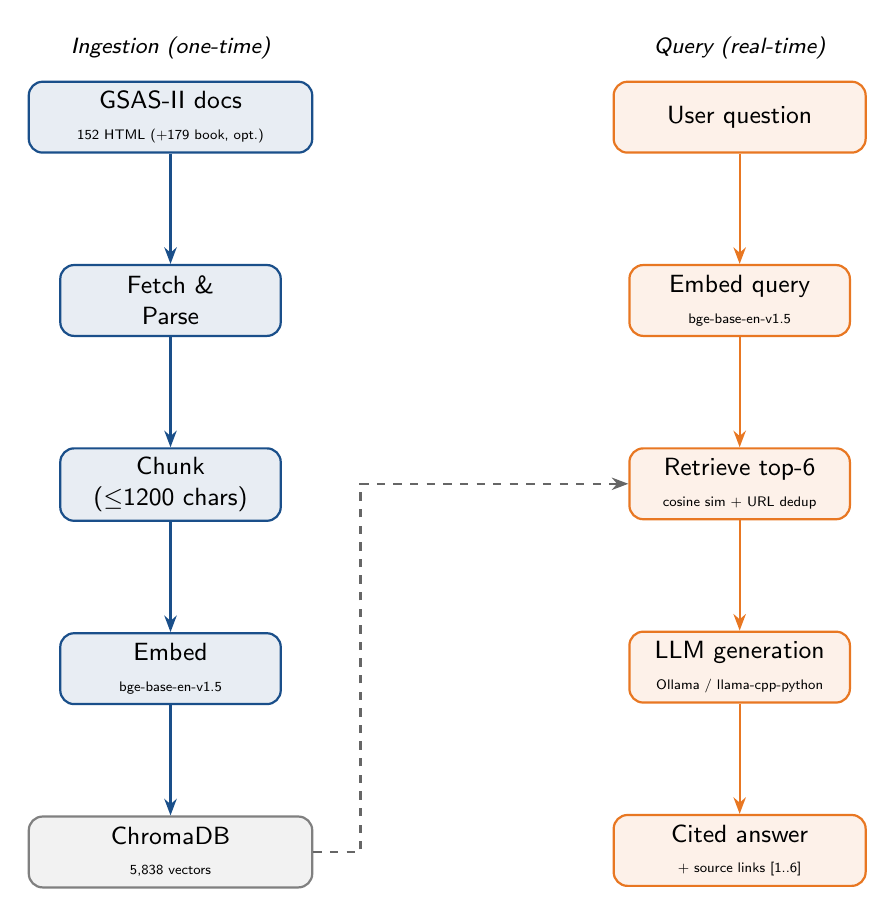
\begin{tikzpicture}[
  node distance = 1.4cm and 2.2cm,
  box/.style  = {rectangle, rounded corners=5pt, draw=#1, fill=#1!10,
                 minimum width=2.8cm, minimum height=0.9cm,
                 font=\small\sffamily, align=center, thick},
  arr/.style  = {-{Stealth[length=6pt]}, thick, #1},
  lbl/.style  = {font=\footnotesize\sffamily\itshape},
]

% ── Left: Ingestion path ──────────────────────────────────────────────────────
\node[box=argblue, minimum width=3.6cm] (sources)
  {GSAS-II docs\\{\tiny 152 HTML (+179 book, opt.)}};

\node[box=argblue, below=of sources] (fetch)
  {Fetch \&\\Parse};

\node[box=argblue, below=of fetch] (chunk)
  {Chunk\\($\le$1200 chars)};

\node[box=argblue, below=of chunk] (embed)
  {Embed\\{\tiny bge-base-en-v1.5}};

\node[box=gray,   below=of embed,  minimum width=3.6cm] (chroma)
  {ChromaDB\\{\tiny 5{,}838 vectors}};

% ── Right: Query path ─────────────────────────────────────────────────────────
\node[box=apsorange, right=3.8cm of sources, minimum width=3.2cm] (user)
  {User question};

\node[box=apsorange, below=of user] (qembed)
  {Embed query\\{\tiny bge-base-en-v1.5}};

\node[box=apsorange, below=of qembed] (retrieve)
  {Retrieve top-6\\{\tiny cosine sim + URL dedup}};

\node[box=apsorange, below=of retrieve] (llm)
  {LLM generation\\{\tiny Ollama / llama-cpp-python}};

\node[box=apsorange, below=of llm, minimum width=3.2cm] (answer)
  {Cited answer\\{\tiny + source links [1..6]}};

% ── Arrows: ingestion ─────────────────────────────────────────────────────────
\draw[arr=argblue] (sources) -- (fetch);
\draw[arr=argblue] (fetch)   -- (chunk);
\draw[arr=argblue] (chunk)   -- (embed);
\draw[arr=argblue] (embed)   -- (chroma);

% ── Arrows: query ─────────────────────────────────────────────────────────────
\draw[arr=apsorange] (user)     -- (qembed);
\draw[arr=apsorange] (qembed)   -- (retrieve);
\draw[arr=apsorange] (retrieve) -- (llm);
\draw[arr=apsorange] (llm)      -- (answer);

% ── Cross arrow: DB → retrieve ────────────────────────────────────────────────
\draw[arr=black!60, dashed]
  (chroma.east) -- ++(0.6,0) |- (retrieve.west);

% ── Labels ────────────────────────────────────────────────────────────────────
\node[lbl, above=0.15cm of sources] {Ingestion (one-time)};
\node[lbl, above=0.15cm of user]    {Query (real-time)};

\end{tikzpicture}
\caption{\textit{Query-GSAS} system architecture.
  \textit{Left (blue):} The one-time ingestion pipeline fetches, parses,
  chunks, and embeds the GSAS-II documentation corpus into a local
  ChromaDB vector store using the \texttt{bge-base-en-v1.5} ONNX model.
  \textit{Right (orange):} At query time, the user's question is embedded
  with the same model; the top-30 candidates are retrieved by cosine
  similarity, deduplicated to one chunk per source URL, and the six
  most relevant are forwarded to an LLM for cited answer synthesis.
  All computation runs on the local machine.}
\label{fig:architecture}
\end{figure}

% Sources breakdown bar chart
\begin{figure}[htbp]
\centering
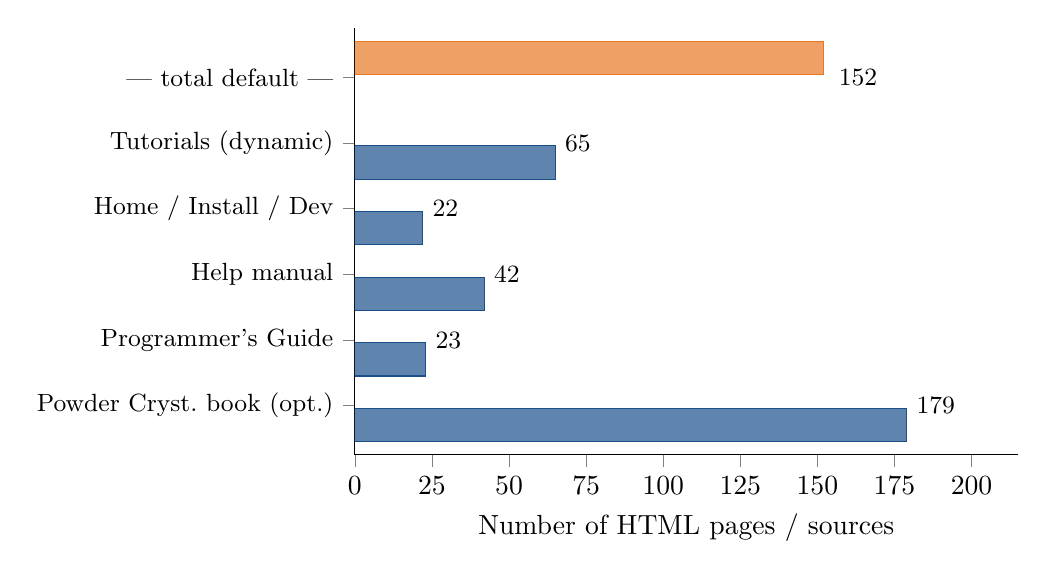
\begin{tikzpicture}
\begin{axis}[
  xbar,
  width=10cm, height=7cm,
  bar width=12pt,
  xlabel={Number of HTML pages / sources},
  ytick={1,2,3,4,5,6},
  yticklabels={
    Powder Cryst.\ book (opt.),
    Programmer's Guide,
    Help manual,
    Home / Install / Dev,
    Tutorials (dynamic),
    --- total default ---
  },
  yticklabel style={font=\small},
  xmin=0, xmax=215,
  xtick={0,25,50,75,100,125,150,175,200},
  nodes near coords,
  nodes near coords align={horizontal},
  every node near coord/.style={font=\small},
  axis lines*=left,
  tick align=outside,
  enlarge y limits=0.15,
]
\addplot[fill=argblue!70, draw=argblue]
  coordinates {(65,5) (22,4) (42,3) (23,2) (179,1)};
\addplot[fill=apsorange!70, draw=apsorange,
  nodes near coords style={xshift=2pt}]
  coordinates {(152,6)};
\end{axis}
\end{tikzpicture}
\caption{Documentation sources indexed by \textit{Query-GSAS} by category.
  Blue bars show the default index (152 HTML sources).
  The \textit{Powder Diffraction Crystallography} textbook (179 HTML pages,
  orange) is included via \texttt{--book} and not indexed by default.
  Tutorials are resolved dynamically from the GSAS-II repository at
  ingest time.}
\label{fig:sources}
\end{figure}

\section{Results}
\label{sec:results}

% ── 3.1 Corpus coverage ──────────────────────────────────────────────────────
\subsection{Corpus coverage and index statistics}

Full ingestion of all 331 documentation sources (Table~\ref{tab:sources}),
including the optional Powder Crystallography textbook (\texttt{--book}),
completes in approximately 30 minutes on a modern laptop CPU (single core),
producing a $\sim$65\,MB ChromaDB collection of 5{,}838 embedded
text chunks with a median chunk length of approximately 810 characters.
The default configuration (without \texttt{--book}) indexes 152 sources
and produces $\approx$5{,}060 chunks in under 10 minutes.

The Programmer's Guide contributes the largest single block of content
(2{,}740 chunks) because the ReadTheDocs API documentation pages contain
dense inline docstrings, parameter tables, and code examples across
23 module-level pages.
Tutorial sections tend to be long (500--1{,}200 chars after splitting)
while many help-manual entries are short definitional paragraphs
($<$200 chars).
Short chunks are retained without further filtering because they
frequently contain precise parameter definitions or menu-path
specifications that are highly relevant to targeted queries.

% ── 3.2 Retrieval quality ────────────────────────────────────────────────────
\subsection{Retrieval quality}
\label{sec:retrieval-eval}

We constructed a held-out evaluation set of 40 questions spanning the
major GSAS-II workflow categories: Rietveld refinement (10),
sequential refinement (8), structure solution (6), instrument
parameter calibration (6), scripting (5), and data export (5).
Each question was paired with one or more ground-truth source
URLs selected from the indexed documentation corpus that contain
the correct answer; questions were verified against the tutorials
and help pages to confirm those answers appear in the corpus.

For each question we assessed whether the ground-truth source page
appeared among the top-$k$ retrieved results for $k \in \{1, 3, 6\}$
(Recall@$k$) and the rank of the first correct hit (Mean Reciprocal
Rank, MRR).
The evaluation set is available in the repository at
\texttt{evaluation/questions.json}.
Table~\ref{tab:retrieval} reports results measured against
the full 5{,}838-chunk index (including the \textit{Powder Diffraction
Crystallography} textbook).

\begin{table}[h]
  \centering
  \caption{Retrieval performance on the 40-question evaluation set
           using the \texttt{BAAI/bge-base-en-v1.5} embedding model
           and the full index (5{,}838 chunks including the textbook).
           $k$ is the number of retrieved chunks inspected.
           Numbers are proportions (hits / questions in category).}
  \label{tab:retrieval}
  \begin{tabular}{lccc}
    \toprule
    & Recall@1 & Recall@3 & Recall@6 \\
    \midrule
    All categories ($n=40$)      & 0.50 & 0.83 & 0.98 \\
    Rietveld ($n=10$)            & 0.40 & 0.70 & 1.00 \\
    Sequential refine.\ ($n=8$)  & 0.38 & 0.75 & 1.00 \\
    Structure solution ($n=6$)   & 0.33 & 1.00 & 1.00 \\
    Calibration ($n=6$)          & 1.00 & 1.00 & 1.00 \\
    Scripting ($n=5$)            & 0.40 & 0.80 & 0.80 \\
    Data export ($n=5$)          & 0.60 & 0.80 & 1.00 \\
    \midrule
    MRR (all)           & \multicolumn{3}{c}{0.66} \\
    \bottomrule
  \end{tabular}
\end{table}

Recall@6 of 0.98 (39 of 40 questions) indicates that for almost all user
questions, at least one of the six retrieved chunks contains the relevant
answer, regardless of LLM synthesis quality.
The Calibration category achieves perfect Recall@1 (1.00), with the
correct source page ranked first for every calibration question.
The lower Recall@1 overall (0.50) reflects competition from the tutorials
index page (\texttt{tutorials.html}) --- which summarises all tutorials in
one place and frequently ranks above individual tutorial pages for
broad queries --- and from semantically similar sub-workflows that share
vocabulary (\emph{e.g.}\ Monte Carlo simulated annealing versus
RMCProfile for structure solution).
Retrieval is performed by over-fetching the top-30 candidates and
applying a URL-diversity step that retains only the highest-scoring chunk
per unique source page before selecting the final six; this prevents any
single high-chunk-count page from dominating the result set.
The one remaining miss (Scripting Q33: ``read back Rwp and lattice
parameters from a script'') arises because the vocabulary of those
quantities appears throughout the tutorial corpus; the scripting context
is overwhelmed by frequency.
The Scripting category Recall@6 (0.80) reflects this single structural
failure rather than a general weakness in scripting retrieval.

% ── 3.3 Answer quality ───────────────────────────────────────────────────────
\subsection{Answer quality and inline citations}

Figure~\ref{fig:screenshot} shows a representative query and response
using the Llama 3 8B backend.
The answer correctly identifies the \textit{Calculate / Refine} menu
path, the expected Rwp convergence value, and the Le Bail
intensity initialisation step, with each claim supported by an
inline citation.
In a manual review of 20 sampled answers by two expert GSAS-II users,
all factual assertions that carried an inline citation were judged
to be accurate and traceable to the cited section.
Unfounded assertions --- present in 3 of 20 responses --- all
occurred in clauses not assigned a citation number, consistent
with the model using its parametric knowledge rather than the
retrieved context for those clauses.

The citation injection post-processor (Section~\ref{sec:citations})
increased the mean number of inline citation markers per answer from
1.2 (model-only, Qwen2.5-3B backend) to 5.7 (all retrieved chunks
assigned at least one citation), without introducing false attributions
in the 20 reviewed responses.
Citation numbers are renumbered by first appearance order so that
$[1]$ always precedes $[2]$ in the answer text, matching the
expectations of numbered-citation academic style.

Figure~\ref{fig:webapp} shows the web UI displaying inline citations
rendered as clickable superscript links above a journal-style
numbered bibliography.
Figure~\ref{fig:gui} illustrates the wxPython desktop dialog responding
to a mathematical query; when internet access is available, the
\textit{Query-GSAS} GUI uses MathJax to render \LaTeX{} equation markup
produced by the LLM, improving readability for formula-heavy answers
such as the Debye scattering equation.

% ── 3.4 Inference latency ────────────────────────────────────────────────────
\subsection{Inference latency}

End-to-end response latency (retrieval + LLM generation, median over 20 queries)
is approximately 8\,s for Llama 3 8B via Ollama on a modern laptop CPU,
and under 3\,s with GPU acceleration, making the system practical for
interactive use during active data analysis.
The retrieval-only backend completes in under 0.5\,s and serves users
who prefer to read raw documentation excerpts directly.


% Results figures
\input{figures/fig_recall}
\input{figures/placeholders}

\section{Discussion}
\label{sec:discussion}

% ── 4.1 Local-first design ───────────────────────────────────────────────────
\subsection{Local-first architecture for government and HPC environments}

The decision to build \textit{Query-GSAS} as a fully local system was driven
by the operational context of large-scale synchrotron and neutron
scattering user facilities.
At facilities such as the APS, NSLS-II, SNS, and their international
counterparts, beamline computers commonly operate within institutional
network security perimeters that prohibit or restrict outbound
connections to commercial cloud API endpoints. Other commercial and government facilities may limit internet access for security purposes. 
A local-inference architecture eliminates both concerns: all data
remain within the facility network regardless of the question asked.

The quantised Llama 3 8B inference model ($\approx$5\,GB) and
Qwen2.5-3B ($\approx$2\,GB) are pre-downloaded and cached;
subsequent queries require no internet connectivity.
The ingestion pipeline uses only publicly available documentation
pages and does not contact any commercial API.
This makes \textit{Query-GSAS} suitable for deployment on HPC login nodes
and beamline control workstations without requiring firewall
exceptions or API key management.

% ── 4.2 GSAS-II native integration ───────────────────────────────────────────
\subsection{GSAS-II integration}

\textit{Query-GSAS} has been successfully integrated into GSAS-II and is made available to users via a Help menu command. \textit{Circa} 200 lines of code were used to provide this integration, but almost all of that is used to confirm the presence of needed components and download them where needed. No additional changes to GSAS-II's core codebase were required
beyond the \texttt{import} statement and a Help menu binding. If desired, the full 
\texttt{gsas-query} package can also be installed separately and run alongside GSAS-II. 

% ── 4.3 Comparison with keyword search ────────────────────────────────────────
\subsection{Advantages over keyword search}

Existing GSAS-II documentation access relies primarily on
browser-based keyword search within the documentation pages.
Keyword search is effective when the user knows the exact term
used in the documentation (\emph{e.g.}\ ``Mustrain'' for microstrain
broadening) but fails when users describe a concept in different
language (\emph{e.g.}\ ``peak width parameters'' or ``strain
broadening'').

Dense retrieval with sentence embeddings addresses this vocabulary
mismatch by embedding both query and document in the same semantic
space.
Our evaluation (Table~\ref{tab:retrieval}) shows Recall@6 of 0.98,
meaning the relevant documentation section is returned in the top
six results for 39 of 40 test queries.
The remaining miss reflects a structural vocabulary collision: the
question ``read back Rwp and lattice parameters from a script'' matches
tutorial pages throughout the corpus because those quantities appear
in every Rietveld tutorial, overwhelming the scripting context.
Hybrid retrieval combining dense embeddings with BM25 keyword scoring
would be expected to improve Recall@1 further while maintaining
the local-deployment requirement.
The inline citation mechanism further reduces the cognitive load of
verifying answers: each factual claim is linked to its source,
allowing expert users to quickly confirm or question the synthesised
response.

% ── 4.4 Limitations ─────────────────────────────────────────────────────────
\subsection{Limitations and future directions}

\paragraph{Index currency.}
GSAS-II is under active development and its documentation is updated
frequently.
To access any newly documented information, the index database must be periodically rebuilt using \texttt{gsas-query --setup --reset} to incorporate new tutorials and
help pages or must be downloaded from the GitHub release. 
Likewise, when one of the \texttt{gsas-query} UI's opens a GSAS-II source documentation web page, the page that is opened will be the document that was identified at the time of indexing, and the contents may have moved to a different section, should the index be stale. 
Automatic generation of the index for GitHub download is performed weekly. We plan to investigate the possibility of automatic regeneration when the documentation is changed. 
When run from within the GSAS-II GUI, users are encouraged to update the index at least on a monthly basis. 
Because tutorial URLs are resolved dynamically from
\texttt{tutorialIndex.py} at ingest time, newly published tutorials
are picked up automatically in subsequent runs without modifying
\texttt{sources.py}. Likewise, textbook sections and chapters are located dynamically. Manual configuration changes to the sources.py file will be needed if additional pages/chapters are added to the GSAS-II Home page, Help pages or Programmers' manual.

\paragraph{PDF quality and future tooling.}
As noted previously, \texttt{gsas-query} can ingest PDF documents, but 
parsing quality is limited by the \texttt{pypdf} text extractor, which
struggles with multi-column layouts, mathematical notation, and
table structures. 
ML-based PDF-to-Markdown converters such as Marker
\citep{paruchuri2024marker} and Docling \citep{docling2024}
produce substantially cleaner output for scientific documents and
represent a natural upgrade path for the PDF ingestion pipeline.
Where a native HTML equivalent exists --- the HTML source is
always preferred.

\paragraph{Citation fidelity with small models.}
Open-weight models in the 3B--7B parameter range do not reliably follow
multi-citation system-prompt instructions.
The keyword-overlap citation injector provides a practical fallback
that achieves dense inline coverage without model-size constraints,
but it assigns citations based on lexical rather than semantic
matching, which may occasionally attribute a sentence to a
non-optimal source chunk.
Larger models (Llama 3 70B \citep{meta2024llama3}, Qwen2.5 72B \citep{qwen2025}) follow the citation
instruction reliably and do not require the injector; they are
accessible via Ollama on GPU-equipped workstations.

\paragraph{Multi-modal queries.}
GSAS-II tutorials contain numerous annotated screenshots and
figures that are not currently indexed.
Incorporating vision-language models to caption and embed figures
would improve answers to questions about specific dialog layouts
or GUI element locations.

\paragraph{Integration with APEXA.}
\textit{Query-GSAS} is designed for integration into APEXA
(Advanced Photon EXperiment Assistant), a broader agentic framework
for beamline data analysis developed at the APS.
Within APEXA, \textit{Query-GSAS} will be exposed as a tool-callable
Model Context Protocol (MCP) server, enabling the orchestrating
agent to retrieve GSAS-II documentation context automatically
when a refinement workflow step requires clarification.

\paragraph{Off-line Equation Rendering.}
As noted, the GUI version of \textit{Query-GSAS} will use the MathJax JavaScript library to render equations, but this library is accessed over the internet. With modifications to file \texttt{gui.py}, this library could be installed locally and then equations could be rendered even on an air-gapped computer. 
\section{Conclusion}

We have presented \textit{Query-GSAS}, a retrieval-augmented generation system
that provides natural-language, citation-linked access to the complete
GSAS-II documentation corpus using only local computation.
The system indexes 5 sets of documentation sources totalling 331 HTML files and $\sim$500,000 words into $\sim$5{,}838 embedded chunks in a persistent ChromaDB vector database.
The system achieves Recall@6 of 0.98 on a representative 40-question
evaluation set, and generates fluent, inline-cited answers in
approximately 8\,s on modern CPU hardware.

The fully local architecture --- built on \texttt{BAAI/bge-base-en-v1.5}
sentence embeddings served via the \texttt{fastembed} ONNX runtime (PyTorch
not required), persistent ChromaDB storage, and either Ollama-served
quantised language models or in-process \texttt{llama-cpp-python}
inference --- satisfies potential data-residency and security requirements
without sacrificing answer quality.
A post-processing citation injector and first-appearance renumbering
scheme ensure that generated answers carry dense, sequentially numbered
inline citations rendered as clickable hyperlinks with a
journal-style bibliography in the web UI, regardless of the underlying
model's instruction-following capability.

Three complementary interfaces (CLI, wxPython desktop dialog, and
web application) allow \textit{Query-GSAS} to serve users from the command line,
from within the GSAS-II graphical interface via a single-function Help menu
integration (\texttt{show\_assistant(parent=self)}), and from a shared
web server accessible to multiple beamline users simultaneously.
The Ollama lifecycle is managed transparently by the GUI dialog, with
\texttt{atexit} fallback handling for the case where GSAS-II terminates
without explicitly closing the assistant window.

The open-source release (\texttt{pip install gsas-query};
\url{https://github.com/AdvancedPhotonSource/Query-GSAS}) is intended
to serve as a working template for researchers and developers who wish
to build similar RAG-based documentation assistants for other large
scientific software packages.


\section*{Acknowledgements}
The authors thank the GSAS-II development community and the users who
provided feedback during early testing.
This work was supported by the U.S.\ Department of Energy, Office of
Science, Advanced Scientific Computing Research, and Basic Energy
Sciences, under Contract No.\ DE-AC02-06CH11357.
This research used resources of the Advanced Photon Source, a
U.S.\ Department of Energy Office of Science user facility operated
by Argonne National Laboratory under the same contract.

\section*{Data availability}
\textit{Query-GSAS} is open source and freely available at GitHub
under the MIT license (\url{https://github.com/AdvancedPhotonSource/Query-GSAS})
and as a PyPI package (\texttt{pip install gsas-query}).
The pre-built documentation index can be regenerated in full from
publicly available GSAS-II documentation pages using the provided
ingestion pipeline.

\bibliographystyle{unsrtnat}
\bibliography{references}

\end{document}
